\documentclass[11pt,a4paper]{article}   % 11 pt text on A4 paper
\usepackage{standalone}                 % \includestandalone, for the diagram composer's drawings

% References
\usepackage{csquotes}                   % quotation marks that follow the document's language
\usepackage[backend=biber,style=apa,natbib=true]{biblatex} % APA 7; compile with Biber
\DeclareLanguageMapping{australian}{british-apa}
\usepackage{xurl}                       % allow long bibliography URLs to wrap within the page
\addbibresource{references.bib}

% Page
\usepackage[margin=25mm]{geometry}      % 25 mm margins all round
\usepackage{parskip}                    % a blank line between paragraphs instead of an indent
\usepackage[australian]{babel}          % Australian hyphenation, and \today as 17 October 2026
\usepackage{iftex}                      % tells which TeX engine is running
\ifPDFTeX                               % for pdfLaTeX only:
  \usepackage[T1]{fontenc}              % proper accented letters, and text that copies cleanly from the PDF
  \usepackage{lmodern}                  % Latin Modern, a crisp scalable version of the default font
\fi                                     % XeLaTeX, LuaLaTeX and Tectonic already use Unicode fonts
\usepackage{microtype}                  % small spacing tweaks so lines break more evenly

% Maths
\usepackage{amsmath}                    % align, cases, matrices and \text inside maths
\usepackage{amssymb}                    % extra symbols such as \mathbb{R}
\usepackage{mathtools}                  % \coloneqq and other fixes for amsmath
\usepackage{amsthm}                     % theorem, definition and proof environments

% Figures and tables
\usepackage{graphicx}                   % \includegraphics, for photos and saved plots
\usepackage{subcaption}                 % sub-figures (a), (b), each with its own caption and label
\usepackage{float}                      % [H] keeps a float exactly where it is written
\usepackage{booktabs}                   % \toprule, \midrule and \bottomrule for clean tables
\usepackage{tabularx}                   % tables that stretch to the line, with wrapping X columns
\usepackage{siunitx}                    % numbers and units: \qty{6.6}{\kilo\watt}, aligned table columns
\sisetup{group-separator={,},group-minimum-digits=4,per-mode=symbol} % 7,790 with a comma, and V/µs
\usepackage{multirow}                   % cells merged down the rows
\usepackage{makecell}                   % a line break inside a cell
\usepackage{threeparttable}             % notes under a table
\usepackage{xltabular}                  % long tables that break across pages, with X columns
\usepackage{tikz}                       % drawing diagrams
\usepackage{pgfplots}                   % charts drawn from data, right in the document
\pgfplotsset{compat=1.18}               % use current pgfplots behaviour (label placement and so on)
\usepackage[american]{circuitikz}       % circuit diagrams; american = zigzag resistors

% Code
\usepackage{xcolor}                     % named colours for the code highlighting below
\usepackage{listings}                   % highlighted code blocks and \lstinline, with no shell-escape
\usepackage{algorithm}                  % numbered, captioned boxes for algorithms
\usepackage{algpseudocode}              % pseudocode commands: \State, \If, \While, \Function, ...
\algrenewcommand\algorithmicrequire{\textbf{Input:}}    % \Require prints Input: rather than Require:
\algrenewcommand\algorithmicensure{\textbf{Output:}}    % \Ensure prints Output: rather than Ensure:
\lstdefinestyle{report}{
  basicstyle       = \ttfamily\small,
  numbers          = left,              % line numbers down the left
  frame            = single,
  breaklines       = true,              % wrap long lines instead of running off the page
  columns          = fullflexible,      % natural letter spacing, not fixed-width columns
  keepspaces       = true,
  showstringspaces = false,
  upquote          = true               % straight quotes, as typed
}
\lstset{style=report}

% Links
\usepackage[hidelinks]{hyperref}        % clickable cross-references and citations, without coloured boxes
\hypersetup{                            % details shown in the PDF viewer's document properties
  pdftitle  = {A stress test for the converter},
  pdfauthor = {Your Name},
  pdflang   = {en-AU}
}
\usepackage[capitalise,noabbrev]{cleveref} % \cref{fig:x} writes "Figure 1.1" for you; load after hyperref

% Number equations, figures and tables by section: (2.1), Figure 2.1, ...
\numberwithin{equation}{section}
\numberwithin{figure}{section}
\numberwithin{table}{section}

% Theorem-like environments, all sharing one counter per section: Theorem 2.1, Example 2.2, ...
\theoremstyle{plain}                    % italic text, for statements
\newtheorem{theorem}{Theorem}[section]
\newtheorem{lemma}[theorem]{Lemma}
\newtheorem{corollary}[theorem]{Corollary}
\theoremstyle{definition}               % upright text, for definitions and examples
\newtheorem{definition}[theorem]{Definition}
\newtheorem{example}[theorem]{Example}
\theoremstyle{remark}                   % italic heading and upright text, for asides
\newtheorem{remark}[theorem]{Remark}
\newenvironment{solution}{\begin{proof}[Solution]}{\end{proof}}

% The document's own commands
\newcommand{\R}{\mathbb{R}}
\newcommand{\vect}[1]{\mathbf{#1}}
\newcommand{\abs}[1]{\left| #1 \right|}
\newcommand{\gain}{A_\mathrm{v}}
\newcommand{\tool}{Spectrum}
\DeclareMathOperator{\tr}{tr}

\title{A stress test for the converter}
\author{Your Name}
\date{3 November 2026}

\begin{document}
\maketitle

\section{Text and references}\label{sec:text}

This document exercises every construct of the house style. \tool{} reads it, and
\cref{sec:maths,sec:floats} hold the maths and the floats. \Cref{sec:code} has the code,
and the units are in \cref{sec:units}.

As \textcite{Masters2013} shows, output follows the sun \parencite{Duffie2013}. A page can
be cited too \parencite[p.~12]{Lamport1994}, and the natbib forms \citet{Knuth1984} and
\citep{Masters2013,Duffie2013} still work, as do \citeauthor{Knuth1984} and
\citeyear{Lamport1994}.\footnote{A footnote with a link to \href{https://example.com}{an example}.}

% A comment on a line of its own comes over as a comment.

Single quotes look like `this', and \enquote{this} is the same. A web address such as
\url{https://typst.app} is a link. Code in a sentence reads \lstinline[language=Python]|heapq.heappop(queue)|,
and a command is written \verb|\cref|.

\begin{itemize}
  \item A bullet point with \emph{emphasis} and \textbf{weight}.
  \item Another, with \textsc{small capitals}.
\end{itemize}

\begin{enumerate}
  \item The first step.
  \item The second step.
\end{enumerate}

\begin{description}
  \item[Term] What the term means.
\end{description}

\section{Maths}\label{sec:maths}

For $\vect{x} \in \R^n$ and a matrix $A$ with $\tr A = 0$, the gain $\gain$ of the stage is
\begin{equation}\label{eq:gain}
  \gain = -\frac{R_f}{R_\mathrm{in}}, \qquad \eta_{\text{ref}} \bigl[ 1 - \beta \, (T_c - T_{\text{ref}}) \bigr].
\end{equation}
The two lines of \cref{eq:first,eq:second} have a number each,
\begin{align}
  x_1(t) &= e^{3t} + e^{-t}, \label{eq:first} \\
  x_2(t) &= e^{3t} - e^{-t}, \label{eq:second}
\end{align}
while this derivation has one number, \eqref{eq:derived}:
\begin{align}
  p(\lambda) &\coloneqq \det(A - \lambda I) \nonumber \\
             &= (\lambda - 3)(\lambda + 1). \label{eq:derived}
\end{align}
Unnumbered displays come in three shapes:
\[
  f(x) = \begin{cases} 1 & x > 0, \\ 0 & \text{otherwise}, \end{cases} \qquad
  \begin{pmatrix} 1 & 2 \\ 2 & 1 \end{pmatrix}, \quad
  \begin{bmatrix} a & b \\ c & d \end{bmatrix}, \quad
  \begin{vmatrix} a & b \\ c & d \end{vmatrix} = ad - bc.
\]
The norm $\left\lVert \vect{v} \right\rVert$, the rank $\operatorname{rank} A$ and $\abs{x - 1}$
read as written.

\begin{theorem}[Euclid]\label{thm:euclid}
There are infinitely many prime numbers.
\end{theorem}

\begin{proof}
Suppose there were finitely many. Their product plus one has a prime factor not in the list.
\end{proof}

\begin{lemma}\label{lem:split}
Every integer greater than one is a product of primes.
\end{lemma}

\begin{corollary}\label{cor:many}
\Cref{thm:euclid} and \cref{lem:split} together give unique factorisation.
\end{corollary}

\begin{definition}\label{def:prime}
A number is \emph{prime} when it has exactly two divisors.
\end{definition}

\begin{example}\label{ex:first}
Find $x$ when $2x = 4$.
\end{example}

\begin{solution}
Divide both sides by 2, so $x = 2$.
\end{solution}

\begin{remark}
Any proof needs only one prime outside the list, as \cref{def:prime,ex:first} suggest.
\end{remark}

\section{Units}\label{sec:units}

Quantities are written with siunitx: a resistor of \qty{4.7}{\kilo\ohm}, a slew rate of
\qty{13}{\volt\per\micro\second}, a supply of \qty{\pm 15}{\volt}, a length of
\qty{1.2 \pm 0.1}{\metre} and a resistance of \qty{47e3}{\ohm}. The old \SI{3.3}{\nano\farad}
still works. A year gave \num{7790} hours of light at a pitch of \ang{22.5}, the panel
reached \qty{65}{\degreeCelsius}, its efficiency was \qty{19.0}{\percent} and the gravity
there is \qty{9.81}{\metre\per\second\squared}. A frequency is in \unit{\hertz}, and a page
is 25\,mm from the edge. In maths a quantity stays text:
$f_c \approx \qty{1.03}{\kilo\hertz}$.


\section{Floats}\label{sec:floats}

\Cref{fig:site} is a photo, \cref{fig:energy} has two panels, \cref{fig:measured} and
\cref{fig:modelled}, and \cref{fig:bode,fig:circuit,fig:amp} are drawn in LaTeX.

\begin{figure}[ht]
  \centering
  
\includegraphics[width=0.5\linewidth,height=0.8\textheight,keepaspectratio]{figures/site}
  \caption{The site, from the north.}
  \label{fig:site}
\end{figure}

\begin{figure}[H]
    \centering
    \begin{subfigure}[t]{0.48\linewidth}
        \centering
        
\includegraphics[width=\linewidth]{figures/measured.png}
        \caption{Measured output.}
        \label{fig:measured}
    \end{subfigure}\hfill
    \begin{subfigure}[t]{0.48\linewidth}
        \centering
        
\includegraphics[width=\linewidth]{figures/modelled.png}
        \caption{Modelled output.}
        \label{fig:modelled}
    \end{subfigure}
    \caption{Energy across the year.}
    \label{fig:energy}
\end{figure}

\begin{figure}[ht]
  \centering
  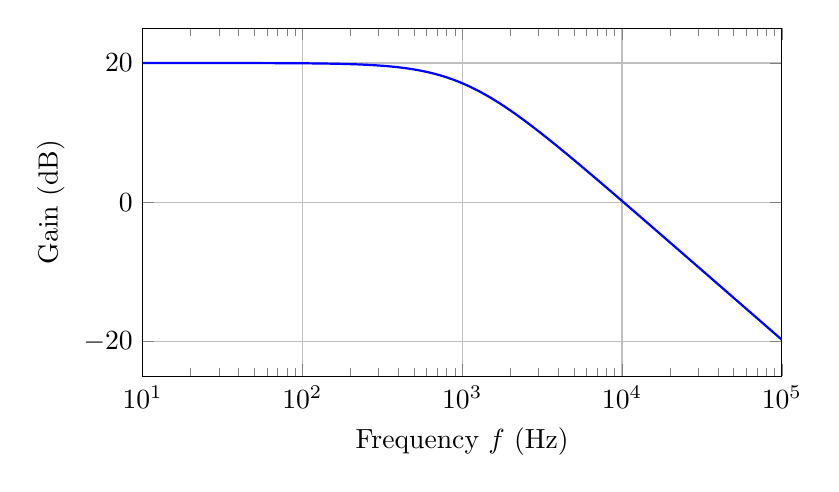
\begin{tikzpicture}
    \begin{semilogxaxis}[
        width=0.8\textwidth, height=6cm, grid=major,
        xmin=10, xmax=1e5, ymin=-25, ymax=25,
        xlabel={Frequency $f$ (\unit{\hertz})}, ylabel={Gain (\unit{\decibel})}]
      % sampled in powers of ten so the points spread evenly along the log axis
      \addplot[thick, blue, domain=1:5, samples=100]
        ({10^x}, {20 - 10*log10(1 + (10^x/1026)^2)});
    \end{semilogxaxis}
  \end{tikzpicture}
  \caption{Gain of the filter: flat at \qty{20}{\decibel}, then falling above $f_c$.}
  \label{fig:bode}
\end{figure}

\begin{figure}[ht]
  \centering
  \begin{circuitikz}
    \draw (0,0) to[R, l=$R_1$] (2,0) to[C, l=$C_1$] (4,0);
  \end{circuitikz}
  \caption{A resistor and a capacitor in series.}
  \label{fig:circuit}
\end{figure}

\begin{figure}[ht]
  \centering
  \includestandalone[width=0.6\linewidth]{diagrams/amp}
  \caption{An amplifier from the diagram composer.}
  \label{fig:amp}
\end{figure}

Two figures can also sit side by side, \cref{fig:left} and \cref{fig:right}, each with its own number.

\begin{figure}[ht]
    \centering
    \begin{minipage}[t]{0.48\linewidth}
        \centering
        
\includegraphics[width=\linewidth]{figures/measured.png}
        \caption{Measured on its own.}
        \label{fig:left}
    \end{minipage}\hfill
    \begin{minipage}[t]{0.48\linewidth}
        \centering
        
\includegraphics[width=\linewidth]{figures/modelled.png}
        \caption{Modelled on its own.}
        \label{fig:right}
    \end{minipage}
\end{figure}

\Cref{tab:seasons} lines its numbers up, \cref{tab:grouped} groups its heading,
\cref{tab:results} has a note, and \cref{tab:parts} stretches to the line.

\begin{table}[ht]
  \centering
  \caption{Energy by season, measured and modelled.}\label{tab:seasons}
  \begin{tabular}{l S[table-format=4.0] S[table-format=4.0] S[table-format=-1.1]}
    \toprule
    Season & {Measured (kWh)} & {Modelled (kWh)} & {Difference (\%)} \\
    \midrule
    Summer & 2740 & 2810 & 2.6  \\
    Winter & 1110 & 1050 & -5.4 \\
    \midrule
    Year   & 7790 & 7790 & 0.0  \\
    \bottomrule
  \end{tabular}
\end{table}

\begin{table}[ht]
  \centering
  \caption{Energy by season, with a grouped heading.}\label{tab:grouped}
  \begin{tabular}{l S[table-format=4.0] S[table-format=4.1]}
    \toprule
    \multirow{2}{*}{Season} & \multicolumn{2}{c}{Energy (kWh)} \\
    \cmidrule(lr){2-3}
     & {Measured} & {Modelled} \\
    \midrule
    Summer & 2740 & 2810.5 \\
    Winter & 1110 & 1050.0 \\
    \bottomrule
  \end{tabular}
\end{table}

\begin{table}[H]
    \centering
    \begin{threeparttable}
        \caption{Results of the two methods.}
        \label{tab:results}
        \begin{tabular}{lc}
            \toprule
            Method & Score\tnote{a} \\
            \midrule
            Ours & 0.91 \\
            \makecell{The method \\ before} & 0.84 \\
            \bottomrule
        \end{tabular}
        \begin{tablenotes}
            \small
            \item[a] Averaged over five runs.
        \end{tablenotes}
    \end{threeparttable}
\end{table}

\begin{table}[ht]
  \centering
  \caption{Parts, with a column that wraps.}
  \label{tab:parts}
  \begin{tabularx}{\linewidth}{l l X}
    \toprule
    Part & Value & Purpose \\
    \midrule
    $R_\mathrm{in}$ & \qty{4.7}{\kilo\ohm} & sets the input current \\
    Op-amp & TL071 & JFET-input op-amp on a \qty{\pm 15}{\volt} supply \\
    \bottomrule
  \end{tabularx}
\end{table}

\Cref{tab:long} may run across pages.
% a comment inside a paragraph stays in it
Its heading rows repeat at the top of each page.

\begin{xltabular}{\linewidth}{lX}
    \caption{Readings, in a table that may break across pages.}\label{tab:long} \\
    \toprule
    Month & Note \\
    \midrule
    \endfirsthead
    \toprule
    Month & Note \\
    \midrule
    \endhead
    \multicolumn{2}{r}{\emph{Continued on the next page}} \\
    \endfoot
    \bottomrule
    \endlastfoot
    January & The highest output of the year \\
    June & The lowest, with the shortest days \\
\end{xltabular}

\section{Code}\label{sec:code}

\cref{lst:python} and \cref{lst:c} are listings, and \cref{alg:dijkstra} is pseudocode.

\begin{lstlisting}[language=Python, caption={Dijkstra's algorithm in Python.}, label={lst:python}]
import heapq

def shortest(graph, start):
    queue = [(0, start)]  # the nearest vertex comes out first
    return heapq.heappop(queue)
\end{lstlisting}

\begin{lstlisting}[language=C, caption={Relaxing an edge in C.}, label={lst:c}]
int relax(int dist[], int u, int v, int w)
{
    return dist[u] + w < dist[v];
}
\end{lstlisting}

\begin{algorithm}[ht]
  \caption{Shortest distances from one vertex.}
  \label{alg:dijkstra}
  \begin{algorithmic}[1]
    \Require a graph $G$ with weights $w$ and a start vertex $s$
    \Ensure the distance $d(v)$ to every vertex $v$
    \State $d(v) \gets \infty$ for every vertex $v$, and $d(s) \gets 0$
    \While{the queue $Q$ is not empty}
      \State $u \gets \Call{ExtractMin}{Q}$ \Comment{nearest first}
      \ForAll{edges $(u, v)$}
        \If{$d(u) + w(u, v) < d(v)$}
          \State $d(v) \gets d(u) + w(u, v)$
        \EndIf
      \EndFor
    \EndWhile
    \State \Return $d$
  \end{algorithmic}
\end{algorithm}

\section{Results}\label{sec:results}

The results in \cref{tab:seasons} agree with \cref{eq:gain} and \cref{thm:euclid}, as
\citet{Duffie2013} expected.


\printbibliography

\end{document}
